\documentclass[../Languages.tex]{subfiles}

\begin{document}
\usec{Ada}\label{sec:ada}

\cd{Ada} is a structured, statically types, imperative, wide-spectrum, and
object-oriented high-level computer programming language, extended from
\cd{sec:pascal} and other Languages. It has built-in language support for
design-by-contract, extremely strong typing, explicit concurrency, offering
tasks, synchronous message passing, protected objects, and non-determinism.
\cd{Ada} improves code safety and maintainability by using the compiler to
find errors in favor of runtime errors. \cd{Ada} is an international
standard; the current version is defined by ISO/IEC 8652:2012.

\cd{Ada} was originally designed by a team lead by Jean Ichbiah of CII
Honeywell Bull under contract to the United States Department of Defense (DoD)
from 1977 to 1983 to supersede over 450 programming languages used by the DoD
at that time. \cd{Ada} was named after Ada Lovelace (1815--1852), who has
been credited with being the first computer programmer.

\subsection{Influence}\label{sub:influence}

\begin{Figure}
  \centering
  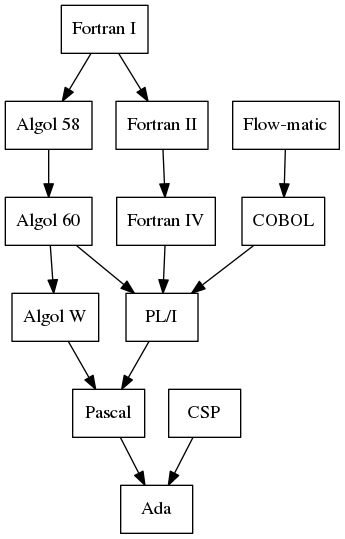
\includegraphics[height=0.5\textheight]{ada}
  \captionof{figure}{Inheritance diagram for \cd{Ada}.}
\end{Figure}

\cd{Ada} was primarily influenced by the languages \cd{Algol}, \cd{Pascal},
\cd{C++}, \cd{Smalltalk}, \cd{Modula-2}, \cd{Java}, and \cd{Eiffel}.

\subsection{Hello World}
\label{sub:hello_world}

\begin{minted}[frame=lines]{ada}
with Ada.Text_IO; use Ada.Text_IO;
procedure Hello is
begin
  Put_Line ("Hello, world!");
end Hello;
\end{minted}

\newpage
\end{document}
